\section{Experiments}
\label{sec:experiments}

We validate through Monte Carlo simulation ($K{=}3$), cross-$K$ robustness checks ($K{=}5,7$), and empirical validation with real LLM confusion matrices from three NLP tasks ($K{=}2,3,10$).

\subsection{Setup}
\label{sec:setup}

For each of the seven topologies (confounding, exposure, mediation, collider, M-bias, front-door, IV), we sample 100{,}000 confusion matrices from a Dirichlet$(1,1,1)$ prior, compute the analytical probability limit of the causal estimator, and validate against Monte Carlo simulation ($N{=}10{,}000$). ASV experiments use $C(\delta) = (1{-}\delta)I + \delta C_0$.

\subsection{Bias Taxonomy}
\label{sec:taxonomy_results}

\paragraph{Theory-MC agreement.}
Analytical probability limits match Monte Carlo estimates with grand MAPE of 1.6\% across 161 scenarios (23 LLM configurations $\times$ 7 topologies, $N{=}10{,}000$). Per-topology MAPE ranges from 0.3\% (confounding) to 3.7\% (IV); the IV maximum reflects the Wald estimator's small-denominator variance amplification.

\paragraph{Exposure DAG: sign reversal under multi-class misclassification.}
Under realistic LLM accuracy (diagonal $\geq 0.7$), the violation rate is 13.7\% with 2.1\% sign reversal; even at diagonal $\geq 0.9$, violation persists at 11.9\%. Under the full Dirichlet$(1,1,1)$ prior, 85\% of $K{=}3$ confusion matrices violate the binary ``toward-null'' guarantee, and 83.4\% cause sign reversal of at least one coefficient. The $K{=}2$ control confirms that all tested binary matrices maintain classical attenuation~\cite{brenner1993}, establishing that the multi-class failure is structurally distinct.

\paragraph{Structural guarantee for non-exposure topologies.}
Five topologies exhibit zero sign-flip rate (Table~\ref{tab:taxonomy}): confounding, mediation, and front-door show 100\% amplification~\cite{brenner1993, dosemeci1990} but never reverse the sign; collider is protective ($|B(C)|$ non-increasing; Conjecture~\ref{conj:monotone}); M-bias shows weakest sensitivity (53.2\% violation). All patterns persist at $K{=}5,7$ (Appendix~\ref{sec:cross_k_robustness}).

\paragraph{IV: Wald estimator instability.}
The IV topology is the sole non-exposure exception: 52.6\% of random matrices cause sign reversal, stable across $K{=}3,5,7$. Under the full Dirichlet$(1,1,1)$ prior, diagonal dominance ($C_{kk} > 0.8$) reduces but does not eliminate IV sign reversal (Appendix~\ref{sec:iv_dirichlet_subspace}); however, across all 23 empirical LLM configurations---including low-accuracy annotators (mean diagonal as low as 0.45)---IV exhibits zero sign reversal. For IV designs where annotation error is unavoidable, practitioners may consider bounds approaches~\cite{manski1990}, robust IV methods, or two-sample designs where the instrument is measured without error in a separate sample.

\begin{table}[t]
\centering
\caption{Bias under $K{=}3$ non-differential misclassification (100{,}000 Dirichlet$(1,1,1)$ matrices). $\tau_{\text{sf}}{=}0$?: sign-flip guarantee holds unconditionally (Yes), conditionally on proportional effects (Cond.; Proposition~\ref{prop:signflip}), or not (No). Amplif.\ denotes $|\hat{\tau}(A^*)| > |\tau|$. For collider, 100\% amplification reflects Berkson bias from conditioning, not error amplification---misclassification is protective (Section~\ref{sec:method}). Violation: $|B| > 0$; Sign Flip: $\operatorname{sign}(\hat{\tau}) \neq \operatorname{sign}(\tau)$.}
\label{tab:taxonomy}
\small
\begin{tabular}{lcccc}
\toprule
\textbf{Topology} & \textbf{Violation} & \textbf{Sign Flip} & \textbf{Amplif.} & $\tau_{\text{sf}}{=}0$? \\
\midrule
Confounding & 100\% & 0\% & 100\% & Cond. \\
Exposure & 85\% & 83.4\% & 14.1\% & No \\
Mediation & 100\% & 0\% & 100\% & Cond. \\
Front-door & 100\% & 0\% & 100\% & Cond. \\
Collider & 100\% & 0\% & 100\% & Cond. \\
M-bias & 53.2\% & 0\% & 10.4\% & Yes \\
IV & 100\% & 52.6\% & 100\% & No \\
\bottomrule
\end{tabular}
\end{table}

The bias distributions are visualized in Figure~\ref{fig:bias_distribution}.

\subsection{ASV Framework Validation}
\label{sec:asv_results}

\paragraph{Envelope monotonicity and magnitude ASV.}
The ASV envelope is $\varepsilon$-approximately monotonic for non-IV topologies ($\varepsilon < 0.06$ under default DGP; Conjecture~\ref{conj:monotone}), confirming $\delta$ as a meaningful severity dial. IV is excluded due to first-stage singularities.
Table~\ref{tab:asv_grid} reports magnitude ASV ranges at $\tau{=}0.5$ with a 10\% bias threshold, ranking from most fragile to most robust: front-door (0.064--0.387) $<$ mediation $<$ confounding $<$ IV (0.101--0.607) $<$ collider (0.338--2.028) $<$ M-bias ($\infty$). M-bias achieves infinite ASV because annotation error only reduces the already-small spurious path.

\paragraph{Significance and sign-flip ASV.}
At $\tau{=}0.05$, significance ASV achieves 100\% power for confounding, front-door, and M-bias, but 0\% for mediation, collider, and IV (correct behavior; Type~I error is 0\%). Sign-flip ASV: 83.4\% of exposure matrices yield $\tau_{\text{sign\_flip}} < 1$; IV ranges 1.1--6.7. The complete ranking (Figure~\ref{fig:asv_ranking}, Table~\ref{tab:asv_grid}, Appendix~\ref{app:supplementary}) confirms IV as maximally fragile and M-bias as immune (ASV $= \infty$).

\paragraph{$N$-sensitivity.}
Significance ASV exhibits a sharp phase transition at $N^* \approx 6{,}000$--$10{,}000$, below which all rejections are blocked. Bootstrap CIs ($B{=}1{,}000$; Appendix~\ref{sec:bootstrap_asv}): $\delta^* = 0.94\,[0.60, 1.36]$ (exposure), $0.75\,[0.44, 1.29]$ (IV); despite wide IV intervals from denominator instability, the topology ranking is stable across all replicates.

\subsection{Empirical Validation}
\label{sec:empirical}

We validate using real LLM confusion matrices from HumAID~\cite{alam2021humaid} ($K{=}10$), VAST ($K{=}3$), and CivilComments ($K{=}2$), with four LLMs producing 23 configurations under zero-shot and few-shot prompting (161 bias scenarios).

\paragraph{Empirical bias ranking.}
HumAID ($K{=}10$) matches predictions: IV (12.4--42.1\%) and exposure (9.0--17.4\%) dominate; remaining topologies $<$15\%. Bias varies substantially across $K$: VAST ($K{=}3$) IV reaches 326\% versus 42\% for HumAID. Across all 56 HumAID scenarios ($K{=}10$), $F_1$ and $|\text{bias}|$ show no significant rank correlation (Spearman $\rho = -0.10$, 95\% CI $[-0.36, 0.17]$, $p = 0.45$; power to detect $|\rho| \geq 0.3$: 0.57; Figure~\ref{fig:f1_vs_bias}).

Of all $K{-}1$ exposure coefficients, 14/23 configurations (61\%) exhibit sign reversal---all in secondary coefficients (Numerical Verification~2); zero across 138 non-exposure scenarios. ASV diagnostics flag 55.4\% of HumAID and 100\% of CivilComments as magnitude-unsafe (Appendix~\ref{sec:asv_diagnostics}).

\begin{figure}[t]
\centering
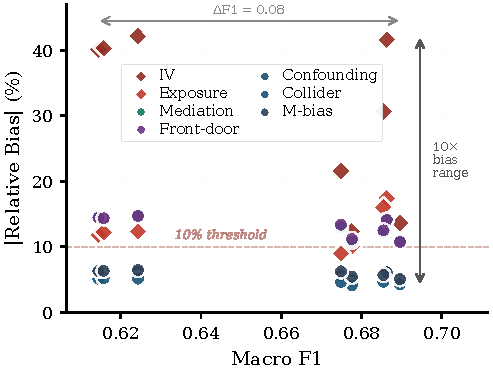
\includegraphics[width=\columnwidth]{fig5_f1_vs_bias.pdf}
\caption{Topology determines downstream causal bias, not $F_1$. HumAID $K{=}10$ (56 points): within $F_1$ range 0.614--0.690, bias varies $10{\times}$ (IV 42.1\% vs.\ collider $<$5.6\%).}
\label{fig:f1_vs_bias}
\end{figure}


\subsection{Correction Guidance}
\label{sec:correction}

We evaluate five correction methods (naive plug-in, MLA, DSL~\cite{egami_hinck_stewart_wei2023}, MC-SIMEX, PPI++~\cite{angelopoulos2023}) across all seven topologies under six error structures (210 configurations; full results in Table~\ref{tab:correction}, Appendix~\ref{app:supplementary}).

\paragraph{FWL invariance.}
Under linear OLS, FWL implies that any linear transformation of $\mathbf{D}^*$ preserves the column space relative to $T$ for the four covariate topologies (where $A$ is a control, not the treatment), so naive plug-in and MLA achieve exactly 0.0\% bias reduction (Appendix~\ref{app:fwl_proof}); exposure and IV are excluded. Under logistic regression the invariance breaks but empirically by $< 0.05\%$ (Table~\ref{tab:fwl_nonlinear}); all structural patterns persist ($|\Delta\,\text{SF}_\tau| < 0.02$; Appendix~\ref{sec:logistic_dgp}).

\paragraph{Method ranking.}
At $K{=}3$, PPI++ achieves the highest grand-mean RMSE reduction (47.0\%) but requires gold labels and is harmful for M-bias ($-$88\%): misclassification attenuates the spurious M-bias path, and PPI++ removes this protective attenuation. PPI++ also degrades with $K$, becoming harmful for exposure at $K{=}10$. MC-SIMEX is more $K$-robust (27--70\% reduction across $K{=}3,5,10$) and gold-free, though it harms front-door ($-$62.4\%). Rankings are stable across $K$ (Spearman $\rho \geq 0.80$; Appendix~\ref{sec:correction_k_sensitivity}); no single method dominates.

\paragraph{Case studies and sensitivity.}
ClinicalBERT validation (Appendix~\ref{app:case_study}) confirms FWL invariance in clinical NLP. PPI++ requires ${\geq}20\%$ gold labels for IV but harms M-bias ($-125\%$ RMSE at 5\% gold; Appendix~\ref{sec:ppi_gold_ratio}). ASV case studies show $3{\times}$ higher error tolerance for confounder vs.\ exposure (Appendix~\ref{sec:asv_case_study}).
